\documentclass[../../thesis.tex]{subfiles}

\begin{document}


\section{Stage 1}

\subsection{Reconstruction}


\subsection{Classification}


\section{Stage 2}


\subsection{Thoughts}

Better inception score and CAS of our models indicate that the class separability learned in latent space makes the conditional distributions more distinct easier to classify. The FID is variable, but in many cases better, which indicated that the generative distributions are closer to the ground truth.\newline

Gaussian noise aug seems to result in a lot easier the BT/VIbCReg loss to minimize. \newline
Slice and shuffle is harder to minimize, but could seem to push representations for different classes further apart resulting in better linear probes.\newline

Talk about the difficulty/ease in minimizing the SSL loss for the different augmentations. Does this affect linear probes / reconstruction / FID / IS / Prior loss
\newline

Mention that during experiments with our stage 2 modification, embed / finetune, we observed that the val prior loss with our modification was higher, but with similar shape as without. If we had time and computational resources to rerun the experiments, then we would omit the stage 2 modification. The FID/IS in our main experiments are in many cases better than baseline VQVAE, despite higher val prior loss.
\newline

For datasets of smaller size with classes of different characteristics (a clear distributional difference in visual inspection [Sony2 and Symbols]) NC-VQVAE seems to perform better both in terms of FID and IS. \newline

The biases introduced by augmentations in stage 1 seems to be included in the generated samples to some degree. In particular datasets with high frequency components, when applying Gaussian noise (easier to spot), has substantially better FID score. 


\subsection{Ablation}

\subsection{Augmentation Reconstruction Weight}
Here are the results of the ablation on the effect of “Augmentation Reconstruction Weight” on Stage 1.
“Augmentation Reconstruction Weight” is the weight given to the reconstruction loss on the augmented branch.
Tested weights $0.05$, $0.1$, $0.15$ and $0.2$.
Augmentations [Window Warp, Amplitude Resize] and [Slice and Shuffle].
The weight has little effect on linear probe accuracy across the four datasets tested, and the two sets of augmentations.
The effect on Validation reconstruction loss is small for all except FordA.
It seems, not very surprisingly, that the choice of augmentations are of (much) greater importance.
\begin{figure}[h]
    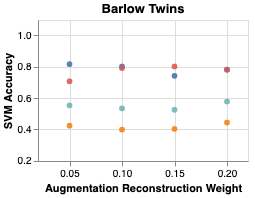
\includegraphics[scale=0.55]{BT_SVM_ReconsWeight.png}
    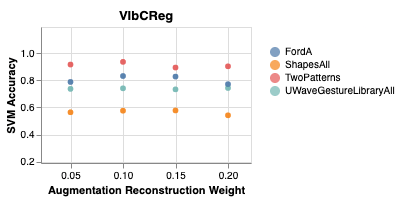
\includegraphics[scale=0.55]{ViB_SVM_ReconsWeight.png}
    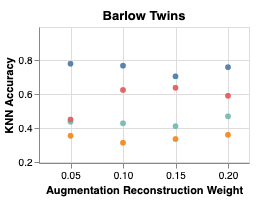
\includegraphics[scale=0.55]{BT_KNN_ReconsWeight.png}
    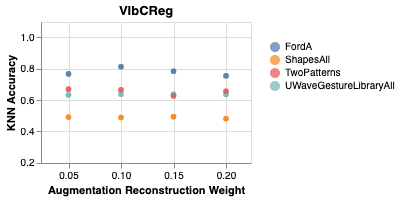
\includegraphics[scale=0.55]{ViB_KNN_ReconsWeight.png}
    \centering  
    \caption{Augmentations: Window Warp and amplitude resize. Averaged across 2 runs. Trained for 250 epochs}  
\end{figure}

\begin{figure}[h]
    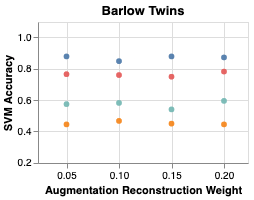
\includegraphics[scale=0.55]{BT_SVM_ReconsWeight_Slice.png}
    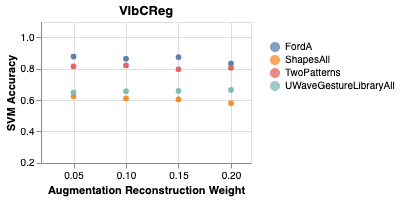
\includegraphics[scale=0.55]{ViB_SVM_ReconsWeight_Slice.png}
    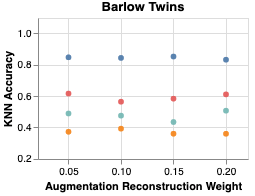
\includegraphics[scale=0.55]{BT_KNN_ReconsWeight_Slice.png}
    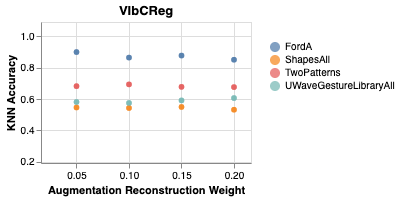
\includegraphics[scale=0.55]{ViB_KNN_ReconsWeight_Slice.png}

    % \centering  
    \caption{Augmentation: Slice and shuffle. Averaged across 2 runs. Trained for 250 epochs}  
\end{figure}

\begin{figure}[h]
    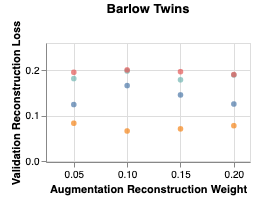
\includegraphics[scale=0.55]{BT_ValRecons_ReconsWeight.png}
    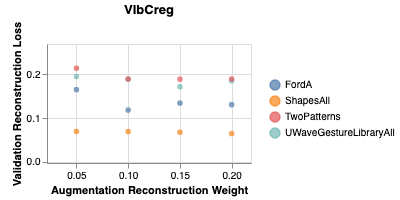
\includegraphics[scale=0.55]{ViB_ValRecons_ReconsWeight.png}
    % \centering  
    \caption{Augmentation: Window Warp and amplitude resize. Averaged across 2 runs. Trained for 250 epochs}  
\end{figure}
\begin{figure}[h]
    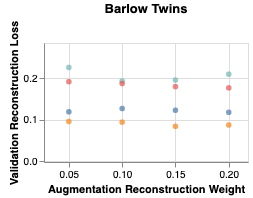
\includegraphics[scale=0.55]{BT_ValRecons_ReconsWeight_Slice.png}
    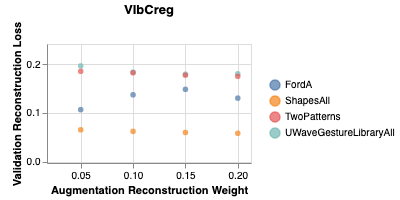
\includegraphics[scale=0.55]{ViB_ValRecons_ReconsWeight_Slice.png}
    % \centering  
    \caption{Augmentation: Slice and shuffle. Averaged across 2 runs. Trained for 250 epochs}  
\end{figure}
\subsection{Augmentation robustness}
\label{section:Augmentation robustness}
S1 - S2 - Augs: Choose datasets such that half were thought to be well fitting for slice and shuffle and half for amplitude resize + window Warp. This was after seeing FordA performing well with S and S, and looking at the augmented views.\newline
FordA/B, Electric devices, ShapesALL for S and S\newline
TwoP, UWave, symbols, Mallat for ampRes + winwarp\newline

Visual inspection: Plot training samples + spectrogram, compare to augmented view. Compare these against others from other classes. \newline
Does the resulting improvement in stage 1 transfer to stage 2? 

\TODO{Download the Wandb data.}
Plot for each dataset and each augmentation: 
Color code according to SSL-model.
\section{Discussion}
The added flexibility of NC-VQVAE, with possibility of choosing dataset specific augmentations, can in some applications be beneficial.\newline


\section{Further work}
\cite{morningstar2024augmentations} suggest that focus on augmentations is of great importance. The hunt for good augmentations in the time series domain is ongoing and should probably get more attention.\newline
HF-LF split - augmentations tailored for HF and LF, as they often have quite different characteristics.\newline
Wavelet transform to improve HF-LF split.\newline

Further optimize the relationship between aug recon loss and choice of augmentations.\newline






\end{document}